\documentclass[11pt]{article}
\usepackage[utf8]{inputenc}
\usepackage[T1]{fontenc}
\usepackage{mathpazo}
\usepackage[margin=1in]{geometry}
\usepackage{graphicx}
\usepackage{xcolor}
\usepackage[colorlinks=true,linkcolor=blue!60!black,citecolor=blue!60!black,urlcolor=blue!60!black]{hyperref}
\usepackage{caption}
\captionsetup{font={small,singlespacing},labelfont=bf}
\usepackage{setspace}
\onehalfspacing

\begin{document}

\section*{Supplemental Figures}

% ---- Figure S1 ----
\begin{figure}[p]
\centering
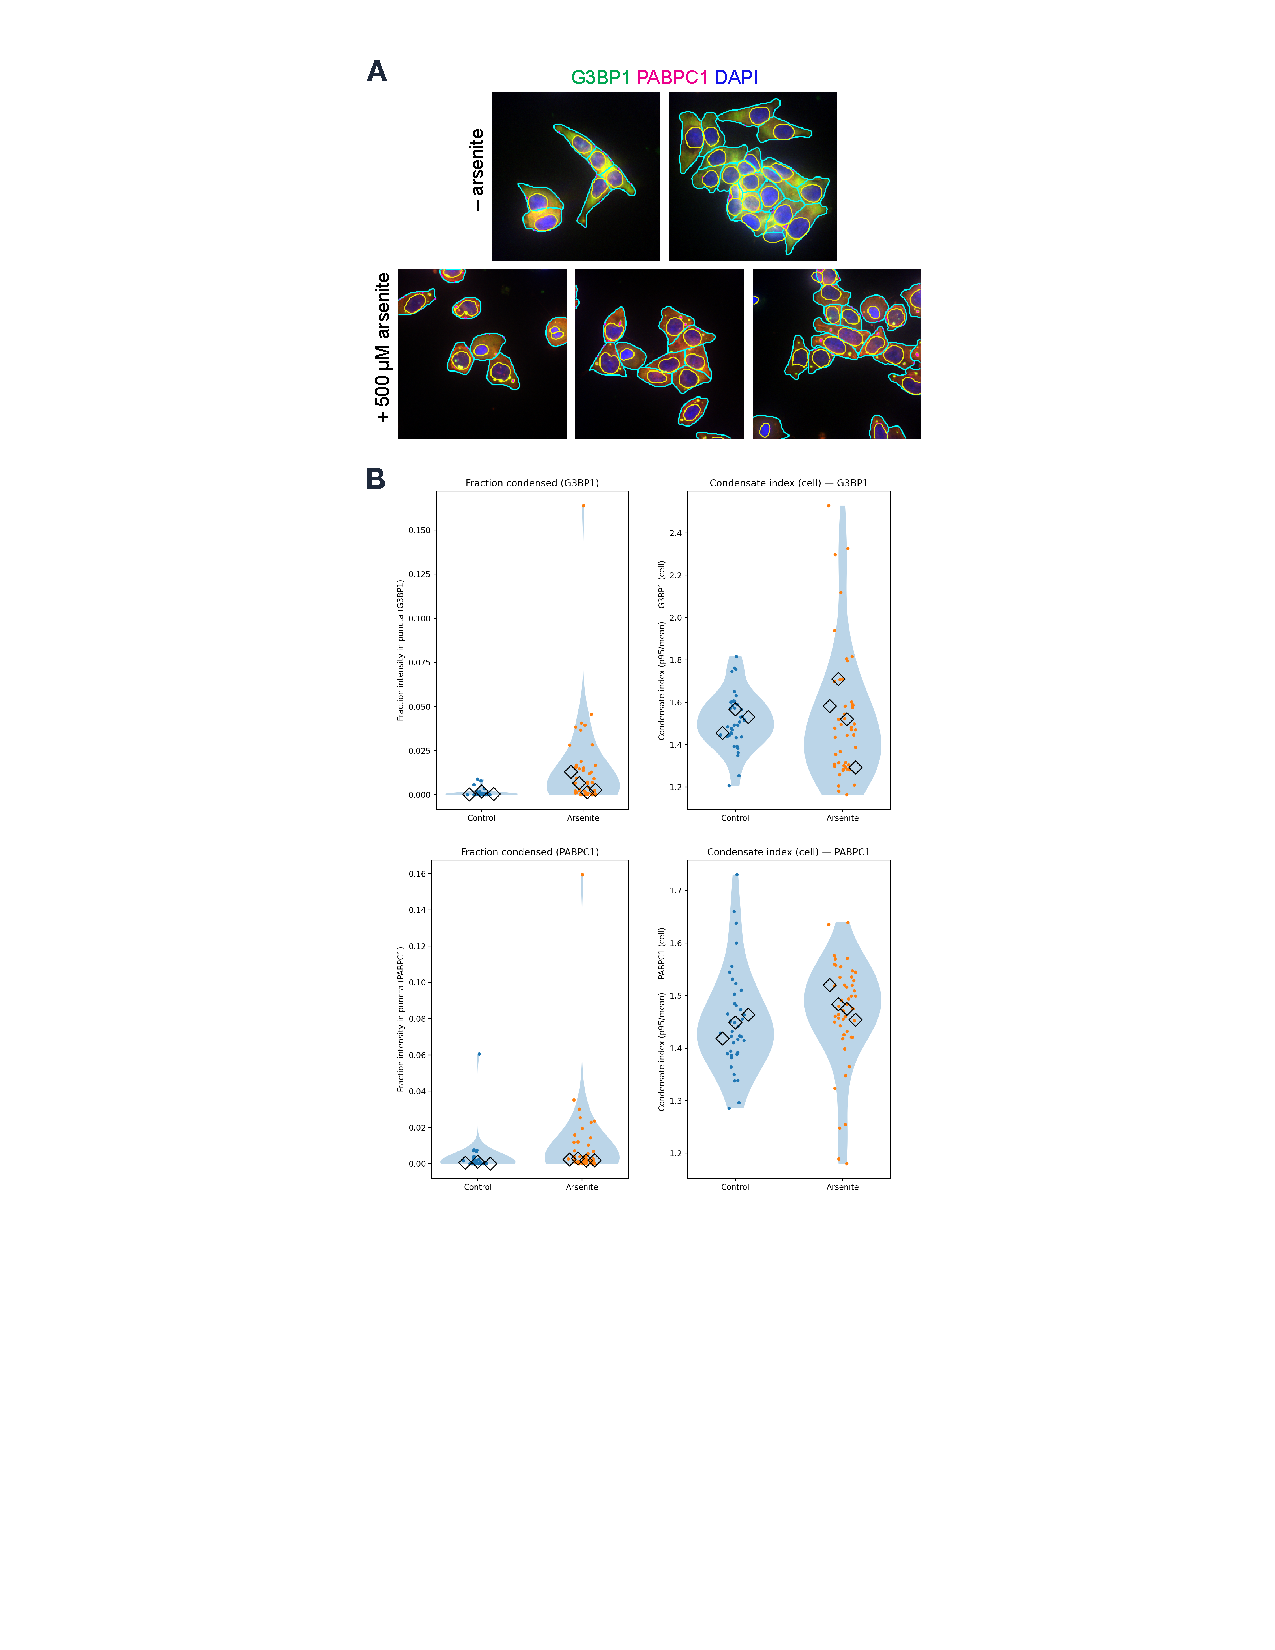
\includegraphics[width=\textwidth]{../FigureS1_U2OS_qc.pdf}
\caption{\textbf{U2OS stress granule quantification.}
\textbf{(A)}~Representative maximum intensity projections of U2OS cells expressing endogenously tagged G3BP1-GFP (green) and PABPC1-mCherry (magenta) with DAPI nuclear stain (blue), untreated (top) or treated with 500~\textmu M sodium arsenite for 1 hour (bottom).
\textbf{(B)}~Superplots showing fraction of signal intensity in puncta (left) and condensate index (right) for G3BP1 (top) and PABPC1 (bottom). Small dots represent individual cells colored by biological replicate; large diamonds indicate replicate means. Violin plots show the distribution of single-cell measurements.}
\label{fig:S1}
\end{figure}

% ---- Figure S2 ----
\begin{figure}[p]
\centering
\includegraphics[width=\textwidth]{../FigureS2_yeast_metrics.pdf}
\caption{\textbf{Comprehensive quantification of yeast condensate and nuclear metrics across the temperature series.}
All metrics were computed by \texttt{cellquant} from three-channel images (Sis1-mVenus, Nsr1-mScarlet-I, Tif6-HaloTag/JF646) acquired at 25\textdegree C, 30\textdegree C, 32\textdegree C, 36\textdegree C, and 40\textdegree C.
Top rows: Manders overlap coefficients (M1) and Pearson correlation coefficients for all channel pairs.
Middle rows: nuclear morphometric parameters (area, circularity, eccentricity, solidity) and condensate indices.
Bottom rows: fraction of signal condensed into puncta, fraction of puncta proximal to the nucleolar marker (Nsr1), mean puncta-to-nucleolus distance, and puncta counts per cell for Sis1 and Tif6.
Each dot represents a single cell; large diamonds indicate per-image means. Temperature conditions are shown on the $x$-axis with individual images as separate groups.}
\label{fig:S2}
\end{figure}

\end{document}
